This chapter describes our approach for generating Puzzle Script levels using different methodologies. Based on the output we conducted our research for generating Puzzle Script rules. This chapter is divided mainly into two parts Level Generation conducted by Rule Generation.

\section{Level Generation}
General Level Generation is not an easy task specially if the main rules can differ from one game. Most of previous work in Puzzle Level Generation (refer to \chref{Chapter3}) was limited for generating levels for a specific game, while the rest just suggest a general technique to be used that is based on designing a game specific fitness function. In this work, we suggest some global metrics for Puzzle Games that can help in generating levels with minimum prior knowledge.\\\par

Our approach relies heavily on the current game rules and objects, and a minimum amount of prior knowledge about Puzzle Script language. \figref{levelGenBlockDiagram} shows a high level block diagram of the system. The following subsections will describe each block in details.

\gfigure{High level system block diagram}{levelGenBlockDiagram}{width=5.5in}{Images/levelGenBlockDiagram}

The system starts by analyzing the current game rules using the Rule Analyzer module. Rule Analyzer module utilize some basic information about Puzzle Script rules to understand the importance of each game object and its basic functionality.\\\par

The output of the Rule Analyzer and the Level Outlines are fed to Level Generator module. Level Generator is responsible for generating initial level layouts. It utilizes the output of the Rule Analyzer to insert every game objects at a suitable position in the Level Outlines. Level Generator uses two different approaches: Constructive Approach and Genetic Approach. Constructive Approach is faster in generation but produce less diverse levels, while Genetic Approach requires more time but give access to a vast majority of levels.\\\par

The generated levels are subjected to a Level Evaluator module. Level Evaluator uses an automated player to play the generated levels. Based on the result of each play, Level Evaluator gives a score for the level based on six different heuristic measures. These measures make sure the resulting level is playable and not trivial.\\\par

In case of Constructive Approach, the system selects the best scored levels to output them, while Genetic Approach, the system enhances the output levels using GA operators.

\subsection{Rule Analyzer}
Rule Analyzer is the first module in the system. It analyzes game rules and extract some useful information about each object. The extracted information is fed to Level Generator and Level Evaluator modules. Each object is assigned:
\begin{itemize}
	\item \textbf{Type:} Each object is assigned a type according to its presence on the Puzzle Script file. There are 4 different types:
	\begin{itemize} \itemsep0pt \parskip0pt \parsep0pt
		\item \textbf{Rule Object:} Any object that appears in a rule is defined as a rule object. Rule objects are essential for rules to be applied.
		\item \textbf{Player Object:} It is defined by name "player" in the Puzzle Script. It is the main game entity. It can move freely without any restriction. Any level must have at least 1 player object to be playable. It must be a Rule Object as well.
		\item \textbf{Winning Object:} They are two object types appearing in the winning condition. At least one of them must be a Rule Object or a Player Object.
		\item \textbf{Solid Object:} All objects that doesn't appear in rules but on same collision layer with at least one Rule Object.
	\end{itemize}
	\item \textbf{Subtype:} By more analysis on Rule Objects and its presence within rules, each Rule Object is assigned a Subtype:
	\begin{itemize} \itemsep0pt \parskip0pt \parsep0pt
		\item \textbf{Critical Object:} If an object presented in a rule with a Player Object and presented with a Winning Object in the same or different rule, it is considered a Critical Object.
		\item \textbf{Normal Object:} It same like Critical Object but only connected to one of them.
		\item \textbf{Useless Object:} It is an object that is neither connected to a Player Object nor a Winning Object.
	\end{itemize}
	\item \textbf{Priority:} It reflects the number of times an object appeared in the game rules.
	\item \textbf{Minimum Number:} The maximum number of times any object appeared in a single rule. For example consider the following group of rules:
	\begin{center}
		[ > Player | Crate ] -> [ > Player | > Crate ]
	\end{center}
	\begin{center}
		[ > Crate | Crate ] -> [ > Crate | > Crate ]
	\end{center}
	The Crate object appeared in both rules. The first rule the Crate object appeared once, while the second rule it appeared twice. That means the minimum number of Crates is 2.
	\item \textbf{Behaviors:} Every object can have one or more behavior. Behavior are analyzed from the difference between left hand side and right hand side of each rule. There are 4 kinds of behaviors:
		\begin{itemize} \itemsep0pt \parskip0pt \parsep0pt
			\item \textbf{Move:} If an object on the left hand side have different movement action associated with it compared to right hand side, this object has Move behavior. For example, In the following rule Crate moves when player approach it.
			\begin{center}
				[ > Player | Crate ] -> [ > Player | > Crate ]
			\end{center}
			\item \textbf{Teleport:} An object is considered to have Teleport behavior if its place in the rule change from left hand side to the right hand side. For example, In the following rule Crate change position with player when it approach it.
			\begin{center}
				[ > Player | Crate ] -> [ Crate | Player ]
			\end{center}
			\item \textbf{Create:} If the number of a certain object on left hand side is less than number of objects on right hand side, then this object have Create behavior. For example, In the following rule, the Crate object is created when Player moves to an empty tile.
			\begin{center}
				[ > Player | \ \ \ \ ] -> [ Crate | Player ]
			\end{center}
			\item \textbf{Destroy:} If the number of certain object on the right hand side is less than number of objects on left hand side, then this object have Destroy behavior. For example, In the following rule, the 3 Crates are destroyed when they are aligned vertically or horizontally.
			\begin{center}
				[ Crate | Crate | Crate ] -> [ \ \ \ \ | \ \ \ \ | \ \ \ \ ]
			\end{center}
		\end{itemize}
	\item \textbf{Relations:} Each object have a list of Relations which contains all objects that appeared in any rule as that object exists. For example, In the following rules, Crate has relations with Player and Lava, Player has a relation with Crate, and Lava has a relation with Crate.
	\begin{center}
		[ > Player | Crate ] -> [ > Player | > Crate ]
	\end{center}
	\begin{center}
		[ > Crate | Lava ] -> [ \ \ \ \ | \ \ \ \ ]
	\end{center}
	A special Relations list for left hand side only is also create at the same time.	
\end{itemize}
\subsection{Level Generator}
Level Generator is responsible for formalizing a level with best possible way to ship it for evaluation. Two approach were used to generate levels.
\subsubsection{Constructive Approach}
Constructive Approach uses information from Rule Analyzer to modify the Level Outlines. In this approach, several levels are generated using an algorithm and the best levels are selected. A pseudo code for the algorithm is presented in \algref{constructiveApproach}.\\

\begin{algorithm}[H]\floatsep20pt \textfloatsep20pt \intextsep20pt
	\KwData{levelOutline, ruleAnalysis, coverPercentage}
	\KwResult{modified level outline}
	\BlankLine
	numberObjects = Get the number of objects for each object type\;
	\BlankLine
	levelOutline = Insert Solid Objects in the level outline\;
	levelOutline = Insert Winning Objects in the level outline\;
	levelOutline = Insert Player Object in the level outline\;
	levelOutline = Insert Critical Objects in the level outline\;
	levelOutline = Insert Rule Objects in the level outline\;
	\BlankLine
	\textbf{return} levelOutline\;
	\caption{Pseudo Algorithm for Constructive Approach}
	\label{Algorithm:constructiveApproach}
\end{algorithm}
The algorithm is consist of two main part. The first part is responsible for determining the amount of objects that should be presented in the current level layout. The second part consists of 5 steps and is responsible for adding the game objects in an intelligent way to the current level.\\\par

\algref{numberObjects} shows the process of calculating the amount of objects. The algorithm starts by determining the percentage that every type should cover from the total number of objects. Each object type must contribute by a percentage equal to the minimum number of objects needed to make all the rules valid. A cover percentage is calculated based on number of critical objects and winning objects. The value of cover percentage is smaller as the percentage of both of critical object and winning object increase and vice versa. Critical Object and Winning Object are the main game objects, without them game may not be playable at all. The increase in there number cause level to be more difficult and more complex. Having small cover percentage when they share huge part of objects, makes sure the game is not very complex.\\

\begin{algorithm}[H]
	\KwData{levelOutline, ruleAnalysis}
	\KwResult{Number of Objects for each type}
	\BlankLine
	percentages[Winning Object] = Minimum Number[Winning Object 1] + Minimum Number[Winning Object 2]\;
	\If{Player Object is a Winning Object}{
		percentages[Winning Object] = 2\;
	}
	percentages[Solid Object] = Number of the different kinds of Solid Objects\;
	percentages[Critical Object] = Summation of Minimum number of all Critical Objects\;
	percentages[Rule Object] = Summation of Minimum number of all rule Objects\;
	Divide all percentages by summation of all of them\;
	\BlankLine
	coverPercentage = 1 - percentages[Winning Object] - percentages[Critical Object]\;
	totalNumber = coverPercentage * total free area in levelOutline\;
	numberObjects = totalNumber * weights * percentages\;
	numberObjects[Player] = 1\;
	\BlankLine
	\textbf{return} numberObjects\;
	\caption{Get the number of objects}
	\label{Algorithm:numberObjects}
\end{algorithm}

The following algorithm all responsible for inserting objects based on numbers from previous part. Most of the Insertion Algorithms needs to find the most suitable empty locations to insert the new Object on it. The most suitable location is based on the object going to be inserted. If the object has a Move behavior, it should be inserted at spots with the most free locations around it. Otherwise any random free location is okay.\\\par

\algref{solidObjects} shows the insertion algorithm for Solid Objects. This algorithm is the first step to modify the level outline. The algorithm just insert random solid objects at a random empty space in the level outline. The algorithm is repeated for several times based on the number calculated from previous step. The same idea is used for inserting Player Object in \algref{playerObject} but only one object is inserted.\\

\begin{algorithm}[H]
	\KwData{levelOutline, ruleAnalysis, numberObjects}
	\KwResult{modified level outlines}
	\BlankLine
	\While{numberObjects[Solid Object] > 0}{
		object = get random solid object\;
		location = Get Suitable Empty Location\;
		levelOutline[location] = object\;
		numberObjects[Solid Object] -= 1\;
	}
	\BlankLine
	\textbf{return} levelOutline\;
	\caption{Insert Solid Objects Algorithm}
	\label{Algorithm:solidObjects}
\end{algorithm}

Before inserting the Player to the level, Winning Objects should be inserted. \algref{winningObjects} is responsible for inserting Winning Objects into the level outline. The algorithm generate an equal amount of Winning Objects except if any of the Winning Objects have Create behavior. The amount of generate Winning Objects must be multiple of minimum number of these objects to ensure that all rules can be applied. The first winning object is inserted at a suitable empty location, while the other is inserted at the farthest suitable empty location. If the Winning Rule is No then the second object must be inserted at same location of the first object.\\

\begin{algorithm}[H]
	\KwData{levelOutline, ruleAnalysis, numberObjects}
	\KwResult{modified level outlines}
	\BlankLine
	\eIf{Winning Objects have Create beahvior}{
		minObject1 = Minimum Number(Winning Object 1)\;
		minObject2 = Minimum Number(Winning Object 2)\;
	}{
		minObject1 = Max(Minimum Number(Winning Object 1), Minimum Number(Winning Object 2))\;
		minObject2 = minObject1\;
	}
	\BlankLine
	\While{numberObjects[Winning Object] > 0}{
		location = Get Suitable Empty Location for Winning Object 1\;
		\For{1 \KwTo minObject1}{
			levelOutline[location] = Winning Object 1\;
			numberObjects[Winning Object] -= 1\;
		}
		\BlankLine
		\If{Winning Rule != No}{
			location = Get the farthest suitable empty location for Winning Object 2\;
		}
		\BlankLine
		\For{1 \KwTo minObject2}{
			levelOutline[location] = Winning Object 1\;
			numberObjects[Winning Object] -= 1\;
		}
	}
	\BlankLine
	\textbf{return} levelOutline\;
	\caption{Insert Winning Objects Algorithm}
	\label{Algorithm:winningObjects}
\end{algorithm}

\begin{algorithm}[H]
	\KwData{levelOutline, ruleAnalysis, numberObjects}
	\KwResult{modified level outlines}
	\BlankLine
	location = GetSuitableEmptyLocation(Player Object, levelOutline, ruleAnalysis)\;
	levelOutline[loction] = Player Object\;
	\BlankLine
	\textbf{return} levelOutline\;
	\caption{Insert Player Object Algorithm}
	\label{Algorithm:playerObject}
\end{algorithm}

\algref{criticalObjects} is responsible for inserting Critical Objects to the level. Critical Objects are one of the most important objects in the game. As they are connected with both Player and Winning Objects. In some games, the game level won't be solvable without Critical Objects. For example, the following rules are from game called DestroyGame. The game goal is to destroy all Gem objects from the level. Gems can be destroyed if it is aligned with 2 other boxes. Boxes can be pushed by the player.
\begin{center} [ > Player | Crate ] -> [ > Player | > Crate ]\end{center}
\begin{center} [ Crate | Gem | Crate ] -> [ \ \ \ \ | \ \ \ \ | \ \ \ \ ]\end{center}
From these rules Crate is a critical object and is the responsible for destroying the Gem. If there is no Crates in the level, the game will be unplayable. For that reason the algorithm ensures inserting Minimum Number of all critical objects. The algorithm adds more random critical objects according to the number required afterwards. Each critical appears based on its Priority feature.\\

\begin{algorithm}[H]
	\KwData{levelOutline, ruleAnalysis, numberObjects}
	\KwResult{modified level outlines}
	\BlankLine
	\ForEach{object in Critical Objects}{
		\For{1 \KwTo Minimum Number of object}{
			location = Get suitable empty location\;
			levelOutline[location] = object\;
			numberObjects[Critical Object] -= 1\;
		}
	}
	\BlankLine
	\While{numberObjects[Critical Object > 0]}{
		object = choose random critical object based on its Priority\;
		\For{1 \KwTo Minimum Number of object}{
			location = Get suitable empty location\;
			levelOutline[location] = object\;
			numberObjects[Critical Object] -= 1\;
		}
	}
	\BlankLine
	\textbf{return} levelOutline\;
	\caption{Insert Critical Objects Algorithm}
	\label{Algorithm:criticalObjects}
\end{algorithm}

Same is done with Rule Objects in \algref{ruleObjects}. As random Rule Objects are inserted to the map based on its priority feature.\\

\begin{algorithm}[H]
	\KwData{levelOutline, ruleAnalysis, numberObjects}
	\KwResult{modified level outlines}
	\BlankLine
	\While{numberObjects[Rule Object > 0]}{
		object = choose random rule object based on its priority\;
		\For{1 \KwTo Minimum Number of object}{
			location = Get suitable empty location\;
			levelOutline[location] = object\;
			numberObjects[Critical Object] -= 1\;
		}
	}
	\BlankLine
	\textbf{return} levelOutline\;
	\caption{Insert Rule Objects Algorithm}
	\label{Algorithm:ruleObjects}
\end{algorithm}

\subsubsection{Genetic Approach}
The second approach used to generate levels for Puzzle Script games. This method uses GA to evolve levels outlines to playable levels. The following points will determine how GA is used to evolve level outlines. Elitism is used to ensure the best levels are sustained.\\\\
\textbf{Chromosome Representation:} GA represents the levels as 2D matrix. The value at each location represents the objects at that location.\\\\
\textbf{Genetic Operators:} Crossover and Mutation are used to ensure better levels in the following generations. One point crossover used where a point (x, y) is selected from the first chromosome and all previous rows (having smaller x) are swapped with the second chromosome. Mutation is different from crossover as it changes any random selected tile using any of the following:
\begin{itemize} \itemsep0pt \parskip0pt \parsep0pt
	\item \textbf{Creating an object:} where a random object is selected to replace any empty tile in the level.
	\item \textbf{Deleting an object:} where a random object from the level is selected to be deleted.
	\item \textbf{Changing the position of an object:} where a random empty tile is swapped with non empty one.
\end{itemize}
The mutation operation happens by subjecting the level to these 3 methods using different probabilities. Creating and deleting an object is subjected to the lowest probabilities compared to changing the position of an object.\\\\
\textbf{Initial Population:} Three different techniques used to test the effect of different Initial Population on the generation process. These techniques are:
\begin{itemize} \itemsep0pt \parskip0pt \parsep0pt
	\item \textbf{Random Initialization:} The population is initialized as a mutated versions of the empty level outline. This technique takes very long time to find a good designed level as it search in the whole space.
	\item \textbf{Constructive Initialization:} The population is initialized using constructive approach algorithm. Using the algorithm tighten the search space so it will not take very long time to find a better level.
	\item \textbf{Mixed Approach:} The population is initialized as a mixture between Random Initialization and Constructive Initialization. A portion of the population is created using the Constructive Approach Algorithm and some mutated versions from its output, while the other portion is the same like Random Initialization. Using that algorithm ensure more diversity than previous two runs.
\end{itemize}
More details about the results of each algorithm will be discussed in the upcoming \chref{Chapter5}.
\subsection{Level Evaluator}
Level Evaluator is responsible for evaluating the generated levels. Evaluating Puzzle Games are based on some heuristic measures. Heuristic measures are based on global knowledge about Puzzle Script games. The first idea was to ensure game playability. That is achieved by using an automated player which we are gonna discuss it later. \figref{diffLevelsSokoban} shows several levels designed for Sokoban game where all are playable but some of them are more interesting than other. The first level is very easy level which can be solve with one move. The second level need more moves which is more interesting than the first level but it is just straight forward toward the solution. The last level is not easy to solve need some prior thinking and trying some moves which is more interesting than previous two.

\gfigure{Examples on different levels for Sokoban game}{diffLevelsSokoban}{width=5.5in}{Images/diffLevelsSokoban}

The above example proves that playability is not enough to judge puzzle levels. Some other metrics must be used to ensure the solution have more moves with some thinking ahead. Six heuristics measures are applied on the output of the automated player to capture this feature.

\subsubsection{Automated Player}
Our Level Evaluator uses a modified version of the BestFS Algorithm as automated player. BestFS Algorithm was introduced in Lim et al.\cite{puzzleScriptGeneration} work. BestFS is similar to BFS algorithm but instead of exploring states sequentially, it sorts them according to fitness function. This causes the algorithm to explore the more important nodes first helping it to reach the solution faster. As explained in \chref{Chapter3}, Lim et al. algorithm uses two metrics to evaluate each game state:
\begin{itemize} \itemsep0pt \parskip0pt \parsep0pt
	\item \textbf{Distance between winning objects:} BestFS tries to either increase or decrease the distance between the winning objects according to the winning rule. The "No" rule is the only rule that need to increase the distance, while the others need to decrease it. \figref{bestFS1} shows an example from Sokoban, where the distance between crates and targets is highlighted.
	\item \textbf{Distance between player and winning objects:} BestFS always tries to minimize the distance between the player and the winning objects. In order to affect the distance between the winning objects, player should come near toward them. \figref{bestFS2} shows same level from Sokoban, where the distance between player and winning objects (crates and targets) is highlighted.
\end{itemize}

\begin{hcfigure}
	\centering
	\begin{minipage}{0.45\textwidth}
		\centering
  		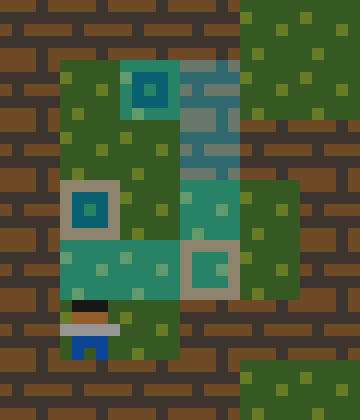
\includegraphics[width=\linewidth]{Images/firstScoreBestFS}
  		\caption{Example of distance between winning objects metric}\label{Figure:bestFS1}
	\end{minipage}\hfill
	\begin{minipage}{0.45\textwidth}
		\centering
  		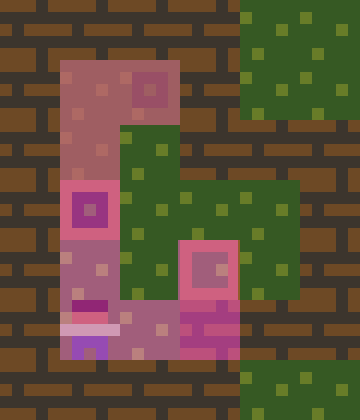
\includegraphics[width=\linewidth]{Images/secondScoreBestFS}
  		\caption{Example of distance between player and winning objects metric}\label{Figure:bestFS2}
	\end{minipage}
\end{hcfigure}

That metric works fine for all games where player is not one of the winning objects. In that case, the two metrics behaves in the same way so the player always try to move towards goal regardless of other game objects. For example, \figref{lavaGame} shows a level from a game called LavaGame. LavaGame is a puzzle game where the goal is to make the player reaches the exit. The path to the exit is usually stuck by lava which can be destroyed by pushing a crate over it. According to the metrics, the player will try to move nearer to the exit by either going left. These movement will not help him to reach the goal, so the player will start wandering aimlessly trying to stumble about a sequence help him reach the goal.

\gfigure{Example level from LavaGame showing the problem in the old metrics}{lavaGame}{width=3.0in}{Images/lavaGame}

Player's aim is to move crates towards lava to unblock his path towards the exit. This aim is somehow explained in the game rules, so by further analysis the game rules we can know which objects need to be closer. Returning to our example about LavaGame, the game rules are stated in the following order:
\begin{center}{[> Player | Crate] -> [> Player | > Crate]}\end{center}
\begin{center}{[> Crate | Lava] -> [ \ \ \ \ | \ \ \ \ ]}\end{center}
The first rule says if there is a player and crate beside each other and the player moves toward it, the crate will also move. The second rule says if there is a crate and lava beside each other and the crate moves toward it, both crate and lava will be destroyed. In any proper game, rules must be applied before achieving the winning condition. Based on that fact, the distance between objects on the left hand side of the rules must be decreased. The new heuristic is the distance between objects in the left hand side of the rules. The relation between objects in the left hand side of the rules is captured by the Rule Analyzer module.\\\par

The three metrics are weighted with respect to each other and used as a new function to evaluate each game state. The weights are chosen by experimentation to ensure best results. The automated player returns four different values that are analyzed and used in the Heuristic measures in the next section. These four values are:
\begin{itemize} \itemsep0pt \parskip0pt \parsep0pt
	\item The score for the best reached state so far. The score is calculated using the first metric (Distance between winning objects). The score value is in range between [0, 1], where the score is equal 1 when a solution is found.
	\item The sequence of movements to reach the best state. The automated player saves up all the movement happens to reach each state.
	\item The number of states explored while searching for the solutions. The automated player increment a variable whenever it explore a new state.
	\item The number of rules that the game engine applied to reach the best state. The game engine increment a variable whenever any of the game rules is applied.
\end{itemize}
The modified BestFS find solution faster than before. More details will be expressed in \chref{Chapter5}.\\\par

\subsubsection{Heuristic Measures}
Heuristic Measure are calculated using a weighted function of six attributes. The function is described as the following:
\begin{center}$F_{score} = 0.3 * P_{score} + 0.2 * L_{score} + 0.15 * N_{score} + 0.12 * B_{score} + 0.12 * R_{score} + 0.11 * E_{score}$\end{center}
where $P_{score}$ is Playing Score, $L_{score}$ is Solution Length Score, $N_{score}$ is Object Number Score, $B_{score}$ is Box Line Score, $R_{score}$ is Applied Rule Score, and $E_{score}$ is Exploration Score. The weights for each attribute are measured experimentally to reflect the importance of some features with respect to the others.
\begin{itemize}
	\item \textbf{Playing Score ($P_{score}$):} Playing score is used to ensure playability of the level. Instead of using a boolean value for playable or not. Score is assigned a value for how much you are near the solution. Automated player is used to play the game and return a value from [0, 1] where 0 means there is no objects at all, while 1 which means the agent reached the solution. Making the domain more continuous helps in measuring the percentage of the level playability. Instead of using it as a constraint to be satisfied.\\\par
	
	Based on the work by Nielsen et al.\cite{gvgpPerformanceProfiles} which proved that Do Nothing player is an important measure for good designed games. A score is calculated for the initial level state and subtracted from the result of the automated player. The heuristic measure can be expressed by the following equation:
	\begin{center}$ P_{total} = P_{score} - N_{score}$\end{center}
	where $P_{score}$ is the automated player score and $N_{score}$ is the Do Nothing player score.
	
	\item\textbf{Solution Length Score ($L_{score}$):} \figref{diffLevelsSokoban} shows that interesting levels usually have more steps than trivial ones. The first idea was to use the length of best movement sequence the automated player has reached and compare it with a required value. This idea will not work as expected because solution length depends on the size of the level. For example, \figref{sokobanLenghtArea} shows different levels from Sokoban and the corresponding solution length. Its obvious that the seconds level have longer solution length than the first one because it have huger area.
	
	\gfigure{Examples of two sokoban levels with different area and solution lengths}{sokobanLenghtArea}{width=4.5in}{Images/sokobanLenghtArea}
	
	From the previous example we can conclude that the solution length depends on the level area. Instead of using the solution length as the metric we used the ratio between the solution length and the level area. A mapping function is need to convert that number to a value in the range [0, 1]. We analyzed 40 hand crafted levels with different area from 5 different games. A histogram is plotted on the collected values of the ratio between the solution length and the level area.
	
	\gfigure{Histogram for the ratio between the solution length and the level area}{solutionLengthHistogram}{width=5.5in}{Images/solutionLengthHistogram}
	
	The histogram in \figref{solutionLengthHistogram} seems to follow a Normal Distribution with $\mu = 1.221$ and $\sigma = 0.461$. Based on that, the Solution Length Score is expressed by the following equation:
	\begin{center}$L_{score} = Normal(\dfrac{L}{A}, 1.221, 0.461)$\end{center}
	where $Normal(ratio, \mu, \sigma)$ is a normal distribution, $L$ is the solution length score, and $A$ is the level area.
	
	\item \textbf{Object Number Score ($N_{score}$):} It is divided into 3 parts:
	\begin{itemize} \itemsep0pt \parskip0pt \parsep0pt
		\item \textbf{Number of Rule Objects:} In a good designed level, most of the rule objects should appear in the level to ensure there is a possibility of applying each rule. The minimum number of times the object should appear in the level must be greater than or equal his minimum number property from Rule Analyzer.
		\item \textbf{Number of Players:} The game should have only one player. If the level have any other value, this part pf the score will be zero.
		\item \textbf{Number of Winning Objects:} The number of the winning objects should be equal, unless one of the winning objects have "Create" behavior. Based on the previous condition, the score is set either to one or zero.
	\end{itemize}
	Object Number Score is calculated using the following equation:
	\begin{center}$N_{score} = 0.4 * N_{rule} + 0.3 * N_{player} + 0.3 * N_{winning}$\end{center}
	where $N_{rule}$ is the Number of Rule Objects, $N_{player}$ is the Number of Players, and $N_{winning}$ is the Number of Winning Objects.
	
	\item \textbf{Box Line Score ($B_{score}$):} It is similar to Taylor and Parberry\cite{sokobanLevelGenerationNew} metric used to find the farthest state. This metric calculates the number of unrepeated moves found in the solution and divide it by total length of the solution. The following equation represents the metric:
	\begin{center}$B_{score} = \dfrac{L_{unique}}{L}$\end{center}
	where $L_{unique}$ is the number of unrepeated moves in the solution and $L$ is the solution length.
	
	\item \textbf{Applied Rule Score ($R_{score}$):} Good level design involves applying game rules number of times to solve a level. The ratio between number of applied rules and solution length should be used for indicting good level design. Exaggerating in applying the rules results in boring level. Same can be said for very low amount of applying. \figref{sokobanRuleScore} shows two levels from Sokoban with different solution. The left level needs to apply Sokoban rule one time to solve the level, while the right needs to apply Sokoban rule with every step.
	
	\gfigure{Example for two boring levels from Sokoban}{sokobanRuleScore}{width=4.5in}{Images/sokobanRuleScore}
	
	To get the calculate the best ratio, We analyzed 40 hand crafted levels with different area from 5 different games. A histogram is plotted on the collected values of the ratio between the number of rules applied and the solution length.
	
	\gfigure{Histogram for the number of rules applied to the solution length}{rulesSolutionLengthHistogram}{width=5.5in}{Images/rulesSolutionLengthHistogram}
	
	The histogram in \figref{rulesSolutionLengthHistogram} seems to follow  Normal Distribution with $\mu = 0.417$ and $\sigma = 0.128$. Based on that the Applied Rule Score can be expressed by the following equation:
	\begin{center}$R_{score} = Normal(\dfrac{R_{applied}}{L}, 0.417, 0.128)$\end{center}
	where $Normal(ration, \mu, \sigma)$ is a normal distribution, $R_{applied}$ is the number of applied rules, and $L$ is the solution length.
	
	\item \textbf{Exploration Score ($E_{score}$):} As the number of explored states increase before reaching goal state this means the level solution is not obvious with the general heuristic. This does not mean exploring huge space without finding a solution is better than exploring small number of states with solution. The following equation express this idea:
	\begin{center}
	$E_{score}= \begin{cases}
	               0.75 + \dfrac{N_{explored}}{N_{max}} & \text{solution exists}\\
	               0.5 & \text{no solution and }N_{explored} = N_{max}\\
	               0 & \text{no solution and }N_{explored} < N_{max}
	           \end{cases}$
	\end{center}
	where $N_{explored}$ is the number of explored states and $N_{max}$ is the maximum number of states the automated player can explore.
\end{itemize}

\section{Rule Generation}
\subsection{Chromosome Representation}
\subsection{Fitness Function}

\tabref{l1}

\tabref{3.1}~demonstrates $\ldots$.

\gtable{Example table for demonstration}{3.1}{width=5.0in}{Table3-1}

\begin{table}[!ht]
	\label{Table:l1}
	\centering
	\begin{tabular}{|c|c|c|}
		\hline
		xxxx & 1233 & ccccc \\
		\hline
		uuuuu & 2323 & gggggg \\
		\hline
	\end{tabular}
	\caption{Example table for demonstration}
\end{table}

\tabref{3.2}.

\begin{landscape}
\gtable{Another example wide table for demonstration}{3.2}{width=9.0in}{Table3-2}
\end{landscape}